\begin{figure}[htbp]\centering
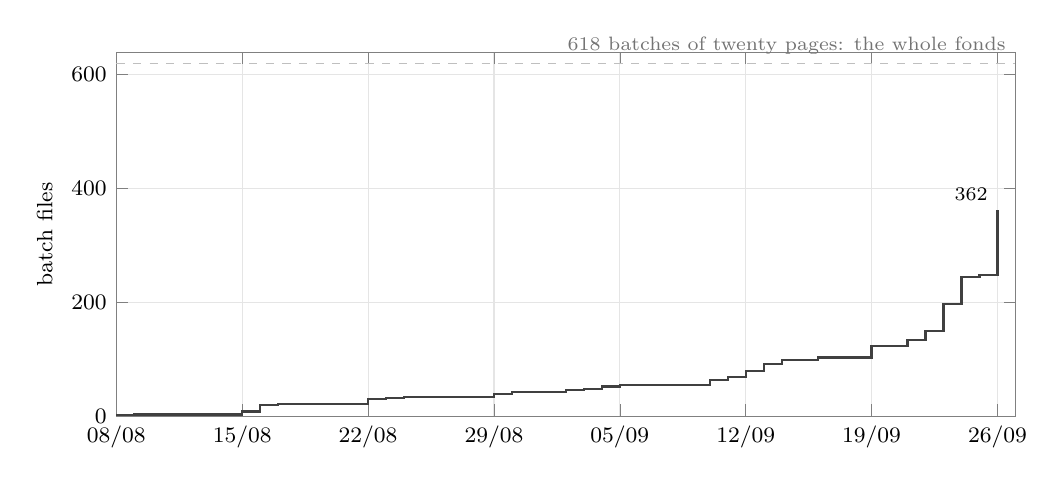
\begin{tikzpicture}
\begin{axis}[width=13cm,height=6.2cm,xmin=0,xmax=50,ymin=0,ymax=638,
  xtick={0,7,14,21,28,35,42,49},xticklabels={08/08,15/08,22/08,29/08,05/09,12/09,19/09,26/09},
  ylabel={batch files},grid=major,grid style={black!10},tick label style={font=\footnotesize},
  label style={font=\footnotesize},axis line style={black!50},clip=false]
\addplot[black!25,dashed,domain=0:50] {618};
\node[font=\scriptsize,text=black!55,anchor=south east] at (axis cs:50,618) {618 batches of twenty pages: the whole fonds};
\addplot[const plot,thick,black!75] coordinates {(0,2) (1,3) (2,3) (3,3) (4,3) (5,3) (6,3) (7,8) (8,20) (9,21) (10,21) (11,21) (12,21) (13,21) (14,30) (15,32) (16,33) (17,34) (18,34) (19,34) (20,34) (21,39) (22,43) (23,43) (24,43) (25,46) (26,48) (27,52) (28,54) (29,55) (30,55) (31,55) (32,55) (33,64) (34,68) (35,79) (36,92) (37,99) (38,99) (39,103) (40,103) (41,103) (42,123) (43,123) (44,133) (45,150) (46,197) (47,244) (48,247) (49,362)};
\node[font=\scriptsize,anchor=south east] at (axis cs:49,362) {362};
\end{axis}
\end{tikzpicture}
\caption{Batch files in the repository, day by day, from the first on 2026-08-08 to 2026-09-26: the date each \texttt{batch-NN.fr.tex} was first committed, cumulated. Each file is one pass of the model over at most twenty pages. The dashed line is the whole fonds at that rate. From the repository's git history, drawn on 2026-09-26 by \texttt{docs/study/figures.mjs}.}\label{fig:pace}
\end{figure}
